\documentclass[12pt, journal, compsoc]{IEEEtran}
\usepackage[utf8]{inputenc}
\usepackage{verbatim}
\usepackage{graphicx}
\usepackage{cprotect}
\usepackage{mathtools}
\usepackage{amsmath}


\title{Social Media Addiction and Repercussions}

\author{Shayan Bathaee}

\date{October 2021}

\begin{document}

\markboth{Social Media Addiction and Repercussions}{}

\IEEEcompsoctitleabstractindextext{
\begin{abstract}
    In this article, we discuss the following subjects relating to social media addiction: Social media history, defining social media addiction, frequency of social media addiction, mental and physical repercussions of prolonged social media use, and company impact. The goal of this article is to bring awareness to those who use social media frequently. 
\end{abstract}

\begin{IEEEkeywords}
    Social Media, Addiction, Mental Health, Psychology, Awareness, Health
\end{IEEEkeywords}}

\maketitle

\section{Introduction}

\hspace{12pt} In the past decade, social media has integrated itself as a part of our society. Now more than ever, we are using social media to stay connected with friends and family. With social media use growing at a rapid pace, researchers in Technological and Psychological fields have started to agree that social media addiction can be classified as a legitimate addiction \cite{UniversityStudents}. In this article, we will examine some of the pitfalls of social media usage in the hopes of bringing awareness to those who use social media frequently. To do so, we will work to define what social media addiction is, figure out how many people are currently addicted, discuss the mental and physical repercussions, and talk about the relationships between large social media companies and their users.

\section{Discussion}
\subsection{Social Media History}

\hspace{12pt} It is widely agreed that the first social networking site was SixDegrees.com \cite{History}. Launched in 1997, this  website was based on the idea that anybody around the world was at most six connections away from each other. The website included features that allowed users to create their own profiles, list their friends, and search for other friends. However, SixDegrees failed to be a sustainable business, and it shut down in 2000 \cite{History}.

From there, the idea of social networking was sparked and various companies started implementing social media aspects into their websites. Online dating, blog, and career sites started popping up from 1997 onwards, with some of the early companies being LiveJournal, Ryze, LinkedIn, and more \cite{History}. 

When researchers discuss the rise of social media, the topic is usually centered around the following three platforms: Friendster, MySpace, and Facebook. These three companies quickly amassed major popularity among their users. Friendster was launched in 2002 to compete with Match.com. Before beginning their planned press coverage for the company in 2003, they already had 300,000 users. However, Friendster ended up having a few significant flaws, including technical difficulties, social collisions, and use restrictions \cite{History}.

When MySpace began in 2003, users who were leaving Friendster quickly got onto the new site \cite{History}. Throughout the following couple of years, MySpace was able to keep up with the demand of users, and make changes to the site to suit their needs. After gaining mass popularity, MySpace was purchased by News Corporation just two years later for \$580 million \cite{History}. As time passed, the company suffered through some safety issues concerning conversations between adults and minors. These problems caused a panic among users, and many left soon after \cite{History}. 

Facebook started in 2004 only supporting networking between students at universities. Because of its beginnings in Harvard, only users with a harvard.edu email address were able to access the website. Facebook was rapidly gaining popularity, so they expanded to various other universities, then to high schools and corporate networks. Soon, anybody was able to make a Facebook account \cite{History}. While many of the social networking sites of this era had a rise and fall, Facebook continued to see growth in their popularity. As of 2021, 2.895 Billion people use Facebook worldwide \cite{MostPopular}.

Current research has shown that approximately 82\% of adults in the United States use some form of social media \cite{TotalUse}. With younger generations integrating online communications into their lives, the number of people using social media platforms is at an all time high \cite{TotalUse}. As the use of these platforms increases,  social media addiction is still being researched and understood. In the upcoming sections, we will examine what we know so far about addictive use of social media.

\begin{figure}[h]
    \noindent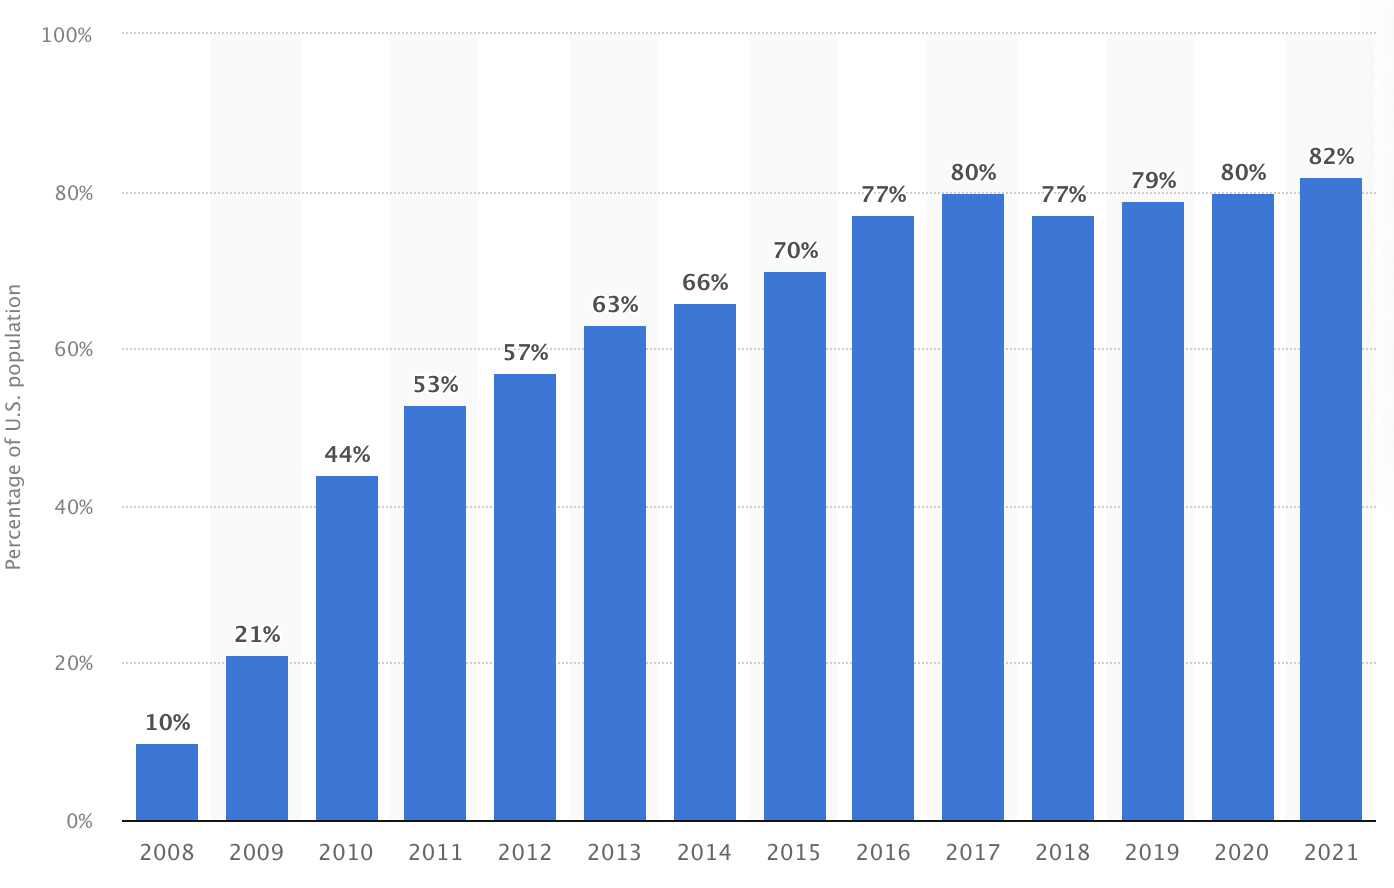
\includegraphics[width = \linewidth]{social media use.png}
    \caption{This chart shows the percent of people in the United States over the age of 17 that use social media \cite{TotalUse}.}
\end{figure}

\subsection{Social Media Addiction}

\hspace{12pt} The first step of defining social media addiction is framing it around the definition of addiction. In the article, \textit{The Relations Among Social Media Addiction, Self-Esteem, and Life Satisfaction in University Students}, Hawi and Samaha write "As we perceive it, social media addiction is the compulsive use of social media sites that manifests itself in behavioral addiction symptoms. The symptoms include salience, tolerance, conflict, withdrawal, relapse, and mood modification" \cite{UniversityStudents}. 

Hawi and Samaha claim that the social media use has increased exponentially, saying that the amount of people using social media is approaching one third of the world's population as of January 2016 \cite{UniversityStudents}. With the number of people joining social media platforms growing so rapidly, they say that keeping up with new research developments is difficult. In their words, "Researchers from different disciplines are barely keeping up with these overwhelming growths, trying to understand the different aspects of social media sites, including descriptive analysis of users, motivations, identity presentation, social interactions, implications, and privacy" \cite{UniversityStudents}. While new developments are hard to keep up with, there are still numerous  recent articles we can use to understand social media addiction. For our cases, we will start with Hawi and Samaha's own research on the correlation between social media addiction, self-esteem, and satisfaction with life.

For their hypothesis, Hawi and Samaha state the following \cite{UniversityStudents}:
\begin{enumerate}
    \item "There is a zero-order correlation between social media addiction and satisfaction with life"
    \item "Self-esteem mediate the relation between social media addiction and satisfaction with life"
    \item "There are no gender differences between social media addiction and self-esteem"
    \item "There are no gender differences between social media addiction and satisfaction with life."
\end{enumerate}

Using a method of systematic random sampling on students at Notre Dame University-Louaize, data was attained via questionnaires on social media use. Of the 364 valid responses, 52.2\% were male. Among the other instruments used to collect data were the Rosenberg Self-Esteem Scale (RSES) and the Satisfaction with Life Scale (SwLS). 

The scores that they received from the questionnaire indicated that their sample had an "overall moderate level of addictive social media use," and "On average, females reported having higher levels of addictive social media use" \cite{UniversityStudents}. The RSES and SwLS results showed high levels of self-esteem and average levels of satisfaction with life. They also showed that females in the test group generally had slightly more self-esteem and are slightly more satisfied with life \cite{UniversityStudents}.

In Hawi and Samaha's discussion, they state that social media users in their sample who reported high levels of social media addiction also had lower levels of self-esteem \cite{UniversityStudents}. They also say that "people with lower self-esteem tend to depend on social media more," and "students who use social media with the intention of enhancing their self-image are at risk of not only lowering their self-esteem but also their satisfaction with life as well" \cite{UniversityStudents}. From this information, we can ascertain that social media addiction can have negative psychological implications. With this high level view of social media addiction, we can continue to explore some of the detailed consequences of problematic social media use.

\subsection{Addiction Prevalence}

\hspace{12pt} Knowing that social media addiction is present, we may want to answer the question: How many people are addicted to social media? Fanni B\'anyai works to answer this question in the article \textit{Problematic Social Media Use: Results from a Large-Scale Nationally Representative Adolescent Sample}. In this research article, B\'anyai surveyed a Hungarian sample of 5,961 adolescents to figure out how many were addicted to social media \cite{ProblematicUse}.

Before showing their results and discussion, the article acknowledges that determining social media addiction prevalence is a very difficult task. According to the researchers in this article, the definition of social media addiction has not been completely solidified \cite{ProblematicUse}. Because of this, there is a lack of assessment tools that can be used to determine if a person is addicted, resulting in conflicting information within the field \cite{ProblematicUse}. 

This is exemplified when B\'anyai says, "For instance, Olowu and Seri [44] reported a prevalence rate of 2.8\% of addicted social media use among college students, while Jafarkarimi and Sim [43] reported a prevalence rate of 47\% being addicted to Facebook among a sample of college students" \cite{ProblematicUse}. Clearly, there has been a lot of misconception about how social media addiction is defined, and what tools we should use to diagnose it. To attempt to solve this problem, B\'anyai first clearly defines social media addiction, and then proposes a standard scale that can be used to test is someone if addicted to social media.

Starting with the definition of problematic social media use, B\'anyai says the following:
\begin{quote}
According to the biopsychosocial model, problematic social media use can be determined by a range of addiction symptoms including: mood modification (i.e., excessive social media use leading to specific changes in mood states), salience (i.e., total preoccupation with social media use), tolerance (i.e., increasing amounts of time using social media), withdrawal symptoms (i.e., negative feelings and psychological symptoms such as irritability, anxiety when social media use is restricted), conflict (i.e., interpersonal problems as a direct result of social media usage), and relapse (i.e., returning to excessive social media use after a period of abstinence) \cite{ProblematicUse}.
\end{quote}

From this, we can see that B\'anyai's definition of problematic social media use is framed around addiction symptoms, similar to the definition that Hawi and Samaha use in their article. 

The next step B\'anyai took to remedy the misconceptions about addiction prevalence was to propose a standard of evaluating social media addiction. To asses the prevalence of problematic social media use, they used a few different scales. First was the Bergen Social Media Addiction Scale (BSMAS), which would be used to determine how addicted the participants were. They also used the RSES, and the Center of Epidemiological Studies Depression-Scale (CES-D) \cite{ProblematicUse}. B\'anyai used these tools to complete the research goal of determining how many people are addicted to social media. Along with this goal, researchers also focused on to verifying that the BSMAS is a reliable scale that can be used to determine one's level of addiction to social media. 

After surveying the participants, the study was able to conclude that the BSMAS was able to accurately identify signs of problematic social media use. Researchers also found that of the 5,961 people sampled, 271 were considered to be at risk of problematic use (approximately 4.5\%) \cite{ProblematicUse}. 4.5\% may not seem like a large number, but apply it to the billions of people using social media, and it is easy to see why this problem is so significant. Along with this, B\'anyai also says that their results are more conservative than most, and that this variance is likely due to other studies having issues such as "convenience sampling, targeting mainly college students, and/or having small sample sizes" \cite{ProblematicUse}.

At the end of the article, B\'anyai concludes that the BSMAS could be a useful tool to determine if adolescents are risk of becoming addicted to social media. The article says, "[BSMAS] could be utilized in prevention and intervention programs (i.e., content-control software, counseling, cognitive-behavioral therapy)" \cite{ProblematicUse}. 

From this article, we can infer that the BSMAS offers an opportunity to clarify some of the questions researchers have been wanting to answer regarding social media use. Along with this, it could be used as a tool to slow down the rapid growth of social media addiction. Another major takeaway from this article is the fact that 4.5\% of the large sample were at risk of social media addiction \cite{ProblematicUse}. Even though B\'anyai says this estimate is conservative, it is still an arguably large size when considering the amount of people using social media today.

\subsection{Repercussions}

\hspace{12pt} All of this information raises the question: What kind of mental and physical repercussions occur when one is addicted to social media? To answer this question, we look at the article \textit{Use of social networking sites (SNSs) and its repercussions on sleep quality, psychosocial behavior, academic performance and circadian rhythm of humans – a brief review}. In this article, authors Rakesh Kumar Swain and Atanu Kumar Pati analyze various detrimental effects of excessive social media to see if the benefits of social networking sites outweigh the cons \cite{Repercussions}. 

The list of negative effects from problematic social media use is quite extensive. To go over all of this information, we will divide it into categories. The first major detrimental effect of social media that this article covers is sleep quality. The article states that there has been a steady decline in the amount of sleep that adolescents get \cite{Repercussions}. Excessive screen usage is a major cause contributing to this decline in sleep quality \cite{Repercussions}. Swain and Pati expand on the impact of insufficient sleep by stating the following: 
\begin{quote}
    Insufficient sleep also leads to the development of negative physiological consequences, including an increased risk of obesity and metabolic dysfunction. Anxiety, depression, mood disturbances, suicidal ideation and drug/alcohol abuse have also been reported among the adolescents due to insufficient sleep (Gupta et al. 2002; Chen et al. 2008; Lowry et al. 2012). Adolescents with poor sleep quality exhibit poor judgment, lack of motivation and decreased life quality \cite{Repercussions}.
\end{quote} 

The article also states that the sleep quality of adolescents who overuse social media is approximately 1.3 times worse than those who whose social media a moderate amount \cite{Repercussions}. Along with the aforementioned problems, there are a plethora of other negative consequences that can arise from lack of sleep. Included in this list are circadian rhythm misalignment, insulin resistance, hypertension, and much more \cite{Repercussions}. From these facts we can infer that the absence of quality sleep is likely to have major detrimental health effects. With excessive screen time being a major cause of sleep deprivation, there is clearly a correlation between these health problems and social media use. 

One of the reasons social media has such a negative effect on both sleep quality and quantity is due to the actual screen itself. Staring at the bright light of a phone/computer screen close to bed time delays the process of melatonin secretion, which is responsible for controlling the sleep cycle \cite{Repercussions}. Thus, looking at screens in the evening directly inhibits one's ability to fall asleep and stay asleep. Due to these factors, Swain and Pati say, "adolescents experience a shift in their biological rhythm and they wake up later in the morning and stay more alert at night" \cite{ProblematicUse}. 



After covering the negative effects that problematic social media use has on sleep, this article talks about social media's relation to psychosocial behaviors. Swain and Pati say that social media use heavily influences many psychosocial behaviors, and can result in some significantly harmful mental effects. It has been shown that overuse of social media can lead to psychiatric distress, depression, anxiety, low self-esteem, lethargic behavior, suicidal ideation, and procrastination \cite{Repercussions}.

This isn't all though. There are many other psychological affects that occur when social media is used too often. Swain and Pati explain some of these effects in the following quote:
\begin{quote}
    Subjects using excessive SNSs [Social Networking Sites] suffer from poor cognitive abilities (Pontes et al. 2018). They also exhibit mood swings and attention deficit (Paul et al. 2012; van Den RJJM et al. 2016; Aalbers et al. 2018). Use of SNSs also induces feeling of loneliness (Kim and LaRose 2009; van Rooij et al. 2017; Barry et al. 2017; Aalbers et al. 2018) and subjective fatigue (Shochat et al. 2010; Aalbers et al. 2018). Many addicted individuals show fear of missing out (FoMo), when they are deprived of  opportunities to use social media (Oberst et al. 2016; Barry et al. 2017; Wegmann et al. 2017; Pontes et al. 2018). Excessive use of SNSs also leads to opioid addiction (Fan et al. 2017) \cite{Repercussions}.
\end{quote}

Researchers say that one of the reasons social media has this big of an impact on mental health is because it causes adolescents to have less face to face interactions \cite{Repercussions}. Many adolescents who use social media spend too much time on it, constantly checking for updates. This in turn causes them to miss out on social activities, and limits their in-person interactions \cite{Repercussions}. In fact, it has been shown that people who use social media too frequently deteriorate their relationships with family and friends, while increasing loneliness and depression \cite{Repercussions}. Heavy social media users often seek clinical evaluations to try to mediate the mental repercussions they face \cite{Repercussions}. Along with these mental health issues, Swain and Pati say that adolescents who frequently use social media also experience "lack of cognitive flexibility (Dong et al. 2014), poor decision making (D’Hondt et al. 2015), anxiety (Wegmann et al. 2015), procrastination (Chóliz and Marco 2012), poor working memory (Dong et al. 2012) and concentration conflicts (Rücker et al. 2015)" \cite{Repercussions}.

Clearly, there are some very serious mental health problems that can occur from using social media too often. These problems can affect every other aspect of the user's life. One particularly concerning result of this is that social media use has been shown to have negative effects on academic performance. To quantify this effect, a study of 1578 students in Ghana showed that students who used social media more often had 20\% lower test scores than those who didn't have social media accounts \cite{Repercussions}. Swain and Pati cited various other sources that come to similar conclusions:
\begin{quote}
    The American Educational Research Association in 2009 at the annual conference in San Diego, California declared that users of social media study less and get low scores (Asif-ur-Rahman et al. 2015). According to Englander et al. (2010), higher the Internet usages among the students lower are their academic scores. They explained this phenomenon as the outcome of the distracted or disruptive aspect of Internet use \cite{Repercussions}.
\end{quote} 

This effect has been attributed to various factors. One being that excessive social media use presents mental and physical repercussions, which inhibit students' studying abilities. Another contributing factor is that students spend a lot more time browsing through social media than they do studying \cite{Repercussions}. As an example of this, the article references a study in San Miguel where students were surveyed on their social media use and academic performance. The students who used Facebook studied 1-5 hours per week, while the students who didn't use Facebook studied 11-15 hours per week \cite{Repercussions}. This difference reflected in their GPAs as well, with non Facebook users getting 3.5 - 4.0, and Facebook users getting 3.0 - 3.5 \cite{Repercussions}. 

Even though there is proof that social media has harmful effects on students' learning abilities, there has also been attempts to integrate social media into learning environments. In some cases, the use of social media has increased certain students' academic performance \cite{Repercussions}. Swain and Pati acknowledge these results by saying, "there are number of reports that did not reveal any negative effects of SNS [Social Networking Site] use on the academic performance" \cite{Repercussions}. However, some researchers believe that integrating social media into classrooms only hurts students, as it exposes them to the negative sides of it as well \cite{Repercussions}. Overall, given the complications surrounding social media addiction and mental health, Swain and Pati agree that there needs to be more research into determining if social media can be a useful academic tool \cite{Repercussions}.

From this information, we can conclude that the ramifications of social media use relating to education are concerning. With social media users having 20\% lower test scores, spending much less time studying, and engaging less with their peers, there are clearly some pitfalls to using social media too often. Although some studies have shown that social media can help in educational settings, a lot more research needs to be done before we can be certain that bringing social media into academics will not be harmful to students.

\begin{figure}[h]
    \noindent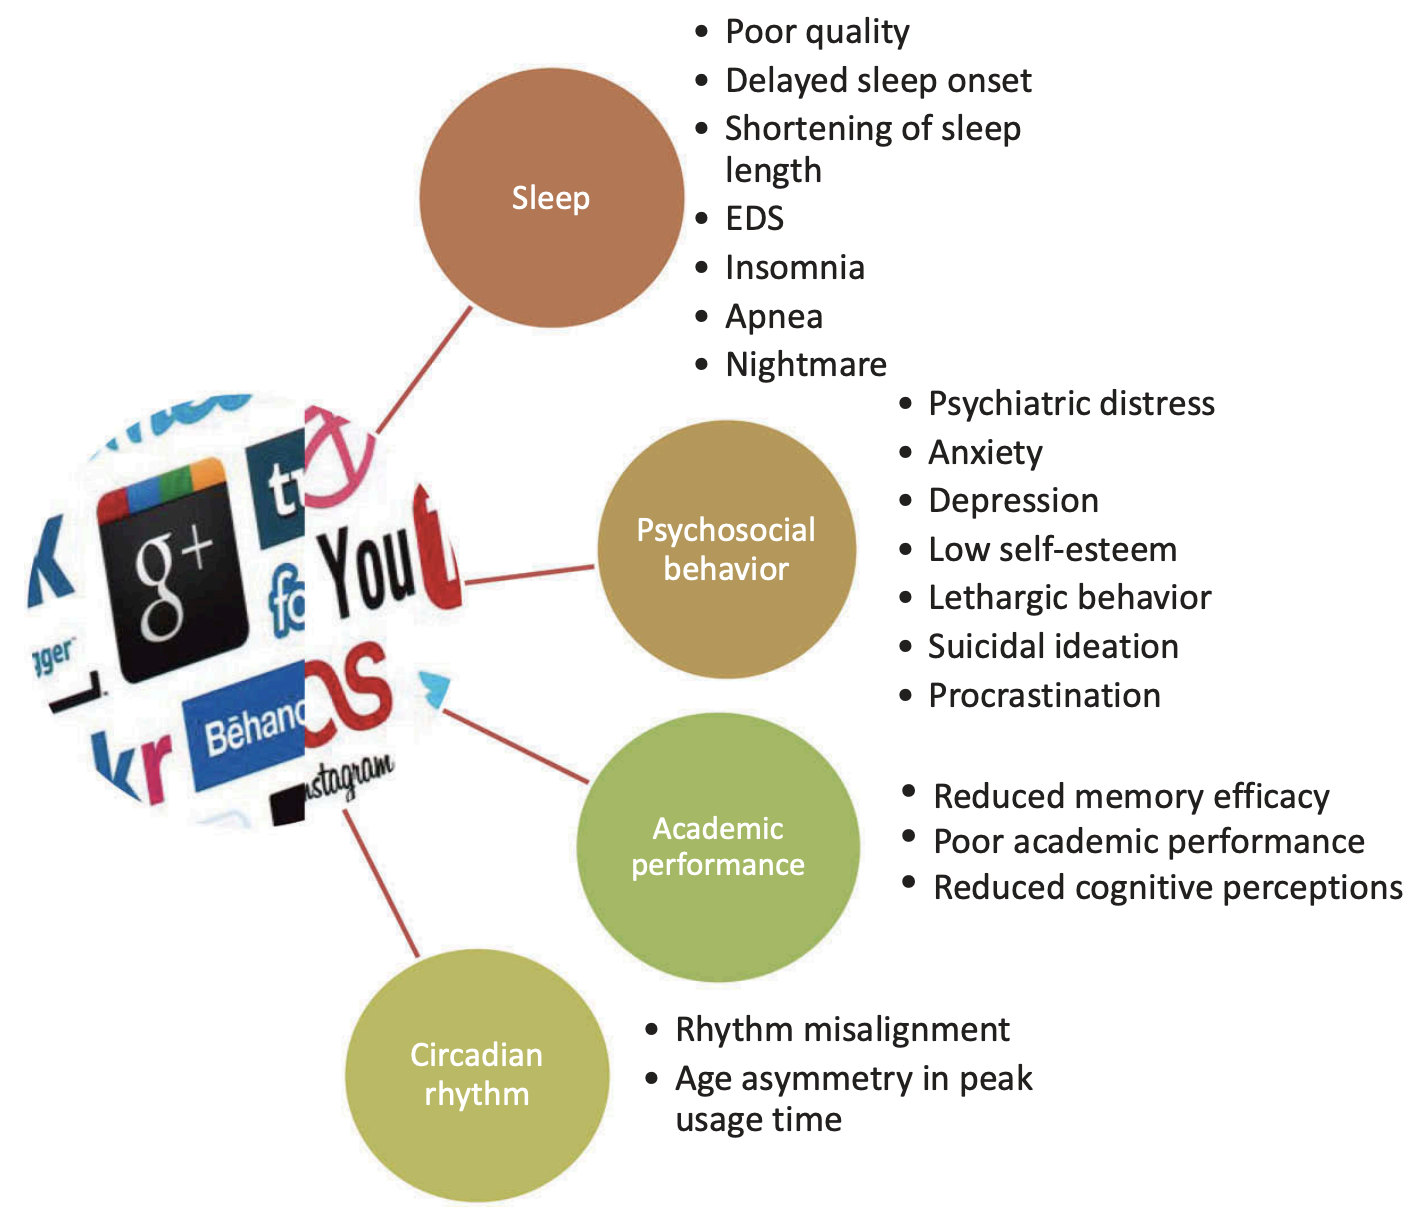
\includegraphics[width = \linewidth]{repercussions.png}
    \caption{This image shows the possible repercussions from social media use divided into different categories \cite{Repercussions}.}
\end{figure}

\subsection{Remedies}

\hspace{12pt} Now that a decent amount of research has been done surrounding social media addiction and it's repercussions, the next point to cover is how social media addiction can be avoided. To do so, we examine the article \textit{Social media addiction: Its impact, mediation, and intervention}. In this study, researchers did a survey on students from Peking University in China \cite{Intervention}. Their goal throughout this research was to examine the relationship between social media, self-esteem, and academic performance. Along with this, they were seeking to understand what tactics are effective at reducing social media addiction \cite{Intervention}.

Because the researchers hadn't yet seen a study of this kind (testing tactics to reduce social media addiction), the first step of the study was to figure out an intervention program for the participants who were social media addicts \cite{Intervention}. To do this, they decided to base their intervention program on previous studies surrounding internet addiction intervention \cite{Intervention}. This led them to the idea of basing their intervention program on self-awareness. They state, "We believe that the cognitive-behavioral approach will be a helpful way to mitigate the negative associations of social media addiction with health and academic outcomes. It will help individuals with social media addiction to recognize their cognitive distortions and further guide them to reconstruct their thinking and behavior" \cite{Intervention}.

For the experiment, they gathered participants who were addicted to social media. Some of the participants were put into a control group, and others were part of the intervention group. The participants in the intervention group partook in a two stage, two week long experiment to reduce their social media addiction. In the first stage, they were asked to reflect on the following \cite{Intervention}:
\begin{itemize}
    \item How much time they spent on social media per day and per week
    \item What other meaningful things they could do with that time
    \item What were the benefits of not using social media
    \item Why did they use social media and were there alternative ways to achieve those purposes
    \item What were the adverse effects of social media use
\end{itemize}
The participants were asked to write down their responses. After reflecting, each participant was given a note card and told to write five advantages of using social media less, and five disadvantages of using social media excessively \cite{Intervention}. After doing so, they were told to take a picture of the card, make it their wallpaper, and put the card on their desks.

In the second stage, the participants were asked to keep a daily record of their thoughts, emotions, and experience in regards to the intervention. Every day before bed, participants would write out things like how they are doing emotionally, what tactics they tried that worked, what they would like to try next, how much they used social media that day, how much they intend on using social media the next day, etc. Each participant was sent a daily reminder to complete their journal entry and send it to the researchers. The responses were not used for collecting any data in the study. They were simply for the participants to become more aware of their use \cite{Intervention}. 

Participants took a survey before and after the intervention to asses their social media addiction. This survey consisted of tests to measure the participants' social media addiction, self-esteem, and mental health. In the end, the results confirmed their hypothesis that the intervention program focused on self-awareness would reduce social media addiction. The participants in the control group saw no significant change in their social media addiction, while the participants in the intervention group saw a significant decrease in their social media addiction \cite{Intervention}. The intervention group also saw an increase in self-esteem, sleep quality, and mental health. The control group made no significant changes in these areas \cite{Intervention}. The authors also added that "participants who received the intervention spent more time on learning and experienced a higher level of learning engagement and better emotional state" \cite{Intervention}.

\begin{figure}[h]
    \noindent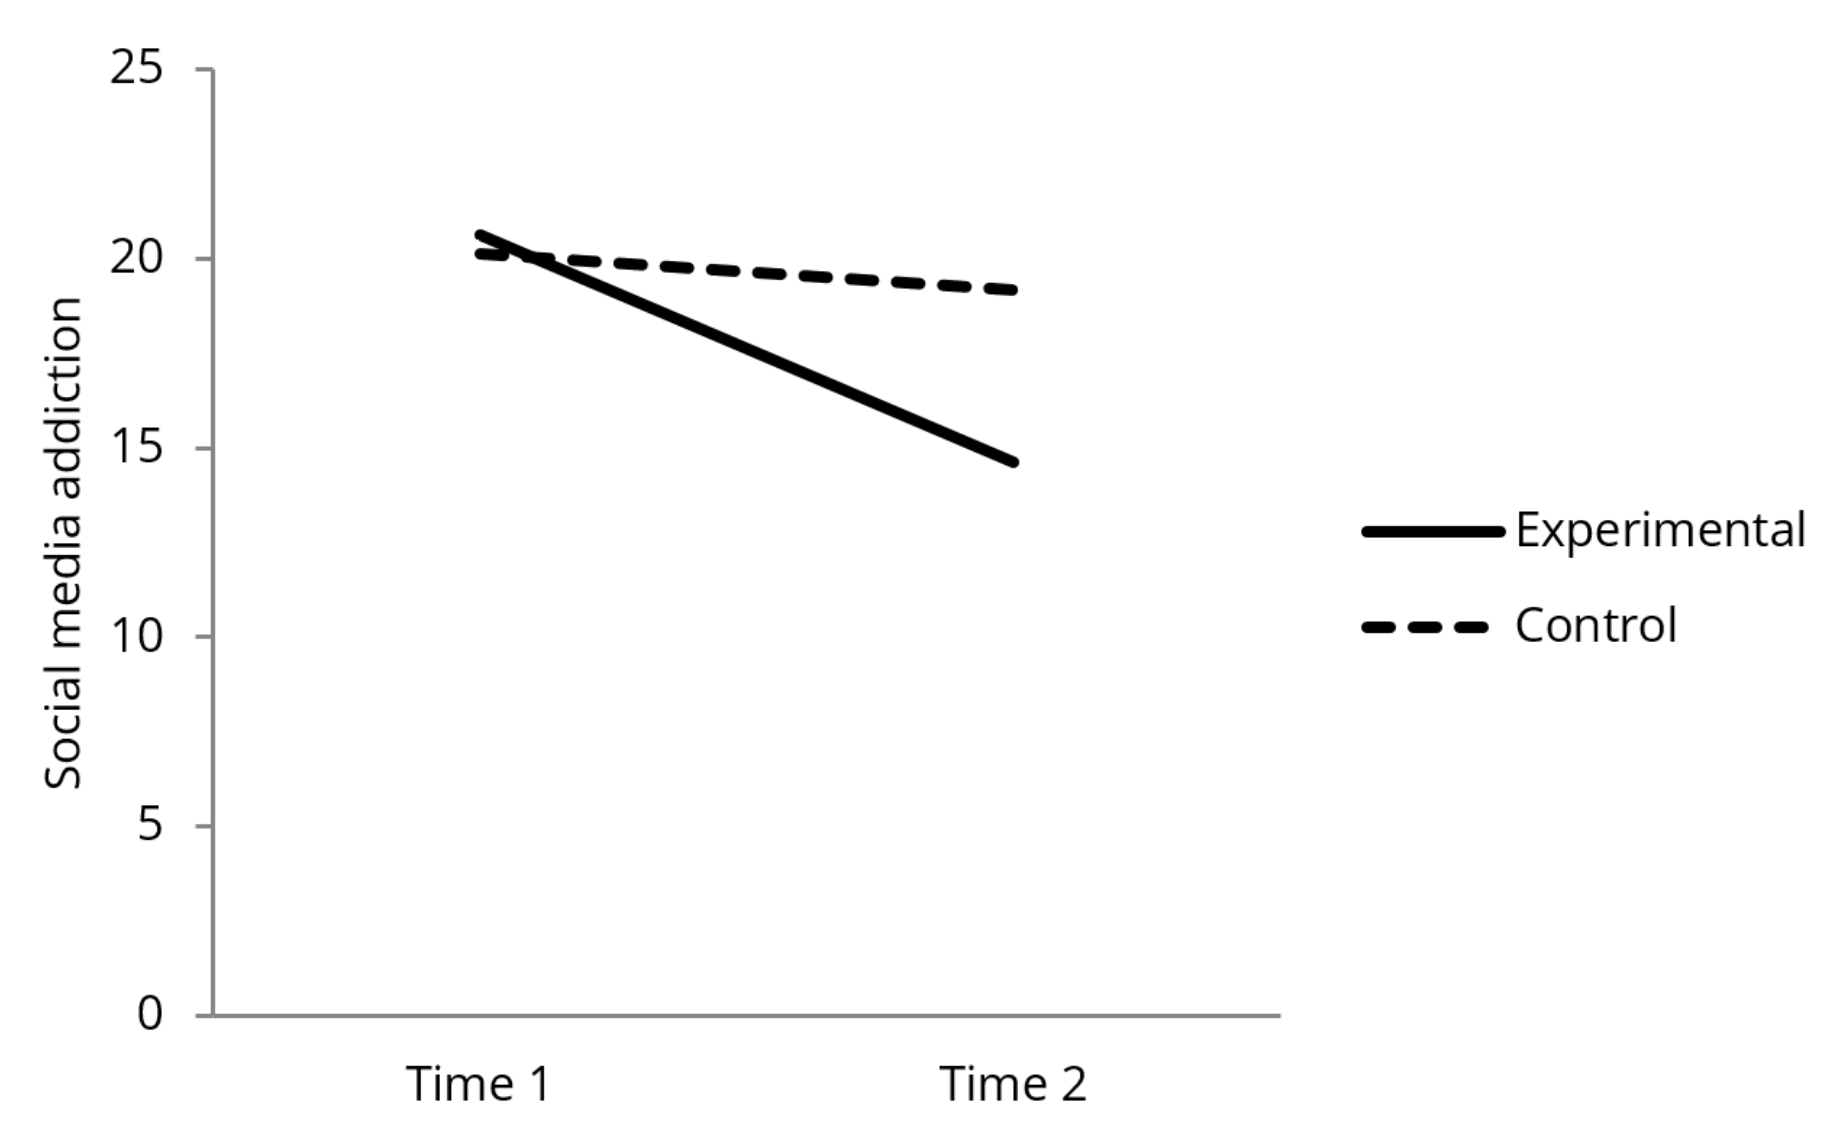
\includegraphics[width = \linewidth]{experiment.png}
    \caption{This graph shows the change in social media addiction for the participants. The control group experienced no significant change, while the intervention group experienced a decline in social media addiction \cite{Intervention}.}
\end{figure}

This study shows that there are still relatively simple ways for people to combat social media addiction by themselves. Simply by taking note of social media habits and setting goals, one can quickly reduce their dependency by a significant amount. In turn, this can result in better sleep, increased learning abilities, better physical health, higher self esteem, higher quality of life, and more. 

\subsection{The Company's Role}

\hspace{12pt} Social media addiction differs than most other addictions in a lot of ways. This is mainly because of the fact that social media companies do not sell a product or service to it's users. In the article \textit{Ethics of the Attention Economy: The Problem of Social Media Addiction}, Vikram R. Bhargava and Manuel Velasquez break this effect down as follows:
\begin{quote}
    With most businesses, the user of the product or service is the source of the revenue. But there is another kind of business—the so-called attention economy business, typically an ad-based business—where the user of the product or service is not directly the source of the revenue. Instead, the user’s attention is the product \cite{Ethics}.
\end{quote}

Knowing this, it's quite obvious that if more people are addicted to social media, the company can generate more revenue. Creators and managers of social media companies know this, and they design their platforms to be inherently addictive \cite{Ethics}. Bhargava and Velasquez say that companies use three main addictive tactics to increase the amount of time users spend on their platforms (and they also note that there are many more besides these three) \cite{Ethics}. First, is the use of "intermittent variable rewards (or what is sometimes called \textit{the slot machine effect})" \cite{Ethics}. An example of this is the 'Pull-to-refresh' feature shown on almost all social media platforms, which "mimics the motion and variable reward schedule of a slot machine" \cite{Ethics}.

Secondly, social media companies take advantage of the human need for social validation, among other psychological needs \cite{Ethics}. For example, Snapchat introduced a "snapstreaks" feature, which keeps track of number of consecutive days two people have messaged each other. Bhargava and Velasquez say, "Teens often face immense pressure to maintain these streaks" \cite{Ethics}. "Like" buttons on social media platforms have also have a significantly addictive effect, and thus most social media platforms have them \cite{Ethics}.

Lastly, many social media companies have gotten rid of natural stopping cues. Bhargava and Velasquez say this "is most prominently seen in the use of infinite scrolls (Harris, 2019; Williams, 2018). Prior to infinite scrolls, when a user arrived at the bottom of a webpage, there was a natural stopping cue ... Now, as the user scrolls, the platform automatically populates the next page" \cite{Ethics}. Because of this, users who are scrolling through their feed have no stopping point. Instead of reflecting on the content they've seen and paying attention to time, users just keep scrolling through the endless stream of content.

The addictive tweaks that have been made to social media platforms does not stop there. Because there are so many people using social media, companies have a large arsenal of testing subjects that they can use to create the most addictive platforms \cite{Ethics}. Companies "run thousands of tests with millions of users to learn which tweaks work and which ones don’t—which background colors, fonts and audio tones maximize engagement and minimize frustration. As an experience evolves, it becomes an irresistible, weaponized version of the experience it once was" \cite{Ethics}.

This raises many ethical concerns surrounding the well being of social media users. Bhargava and Velasquez argue that due to the harm that social media addiction causes, it is ethically wrong for companies to apply tactics that increase addiction among its users \cite{Ethics}. Companies could very easily implement tools that promote the well being of their users, but instead they continue to tweak their platforms to become more addictive. Also, there has been a lack of government policies that prevent social media addiction. There is still a lot of work that could be done by managers of social media companies, policy makers, and educators that could reduce the effect of social media addiction \cite{Ethics}.

\section{Conclusion}

\hspace{12pt} With social media becoming such a prominent part of our lives, it is important that we consider how dangerous social media can be. With social media addiction having negative side effects such as sleep deprivation, depression, and  suicidal ideation, social media users need to be careful and aware of their own habits. Thankfully, we know now that there are ways to reduce social media addiction through tactics that make users self-aware.

A lot more research needs to be done surrounding social media, given the fact that the technology is relatively new and influences so many people. With more knowledge on the positive and negative effects of social media, we can make better decisions on safe social media practices. As the use of social media increases, we need to make sure that research keeps up. If it does, the result could be extremely beneficial for all people, as it would allow us to safely use social media for its intended purpose: Connecting people around the world.

\bibliographystyle{IEEEtran}
\bibliography{refs}

\end{document}
